%%%%%%%%%%%%%%%%%%%%%%%%%%%%%%%%%%%%
\newcommand{\setSinkAgents}[2]{\setSymbol{SG}{#1}{#2}}
\newcommand{\formalAgentResources}[2]{
	\functionFormal{ar}
	{\setAgents{}{} \times \setResource{}{}}
	{\setRealNumbersNonNegative{}{}}
}
\newcommand{\functionAgentResources}[2]{
	\functionSignature{ar}{\varAgent{}{}, \varResource{}{}}
}
\newcommand{\formalSinkMapping}[2]{
	\functionFormal{sg}
	{\setCompositeTask{}{}}
	{\powerSetSymbol{\setSinkAgents{#1}{#2}}{}{}}
}
\reviewquestionopen{Figure 2 seems inconsistent with the text early in the section.
	- How can there be nodes that are distinctly 'sensor nodes' when you say every node has 'one or more sensors'? When you say "...a final measurement is made by a sensor node" do you mean "a sensor node *for that task*", i.e. it is a role played for a given task rather than a distinct kind of node?  If it is meant to be a role within a task, 'sensor node' sounds like a type rather than a role, so there may be a better name to use.
	- When every node has an agent by your definition, then why are some elements in the figure called nodes and others (apparently of the same kind) called agents? 
	- Why does one agent (and possibly by implication other agents) have a 'broadcast radius of node' shown, but this broadcast radius is not mentioned as a property of an agent or node in the text?}


\begin{figure}
\centering 
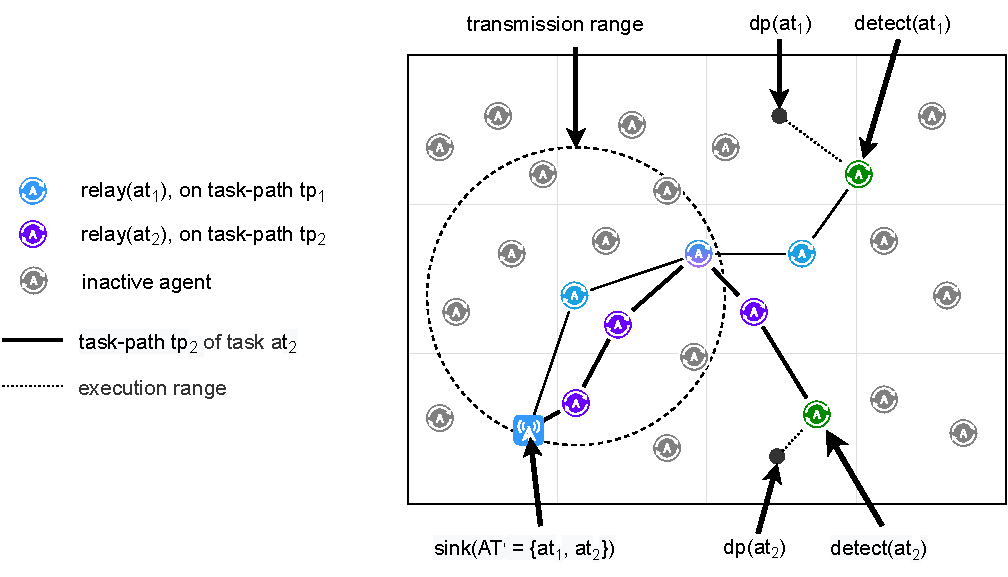
\includegraphics[width=0.9\linewidth, trim={25pt 0pt 24pt 0pt, clip}]{grid_concept}
\caption[WSN deployment terminology]{WSN components and terminology}
\label{fig:grid_concept}
\end{figure}

\subsection{Tasks and resources}
\label{section:tasks}
\reviewquestionopen{In multiple places, there seems confusion between 'agents' and 'nodes', e.g. in paragraph 1, it seems odd to say that the deployment configuration maps agents to locations when agents are 'ethereal' software. Shouldn't it be nodes that are mapped to locations? Or in the system definition, you say "sink nodes, agents the can receive composite tasks" as if nodes are the same as or a subclass of agents which contradicts what you said in Section 3.1.
}
\reviewquestionopen{You need to decide whether you need two distinct concepts with different terms (node for the hardware, agent for the software) or one term because the distinction doesn't matter for your paper. If you have two distinct concepts, then you can't use the terms interchangeably: they refer to different things. If you don't want to distinguish then you need to (a) say that's what you're going to do (e.g. in Section 3.1 say that the distinction between agents and nodes is not important so you will use 'agent' from now on), and (b) only use your chosen term and not the other.
}
\reviewquestionopen{Paragraph 1: "them being either executed" should be "then..."
}
\reviewquestionopen{Paragraph 1: You say that completing atomic tasks requires resources, but you do not mention whether communication between agents requires resources. This feels like an obvious reviewer question: either say that it does or say why it is OK to not include that in the model.
}
\reviewquestionopen{You say "We define the agent-based system..." but to clarify I think you mean "... at an instant of time"? That is, it is a state of the system rather than the persistent system structure? Otherwise, ra couldn't change for example. Alternatively, you could separately define a 'system' as the definition of a system structure containing all the constant elements of your current definition and a time-dependent 'system state' containing the dynamic elements.
}
\reviewquestionopen{When you say "Completing atomic tasks requires resources, such as energy, of which a node has a fixed amount" it is ambiguous what you mean by 'fixed amount'. As a reader I would naturally assume, given your discussion of irreplaceable batteries and energy usage in Section 2, that each node has 'a given initial amount' which reduces as it performs each task - but does 'fixed' then mean that every node has the same initial amount? Or you could mean that it always has the same amount because whenever it uses energy it is replaced somehow - so each node effectively has infinite energy but only a certain amount to pump into something at any one instant. Either way, you need to clarify.
}
In our assumed system there is a geographical area to monitor on which a set of nodes controlled by agents $\setAgents{}{}$ are distributed randomly, such as occurs in an aerial deployment \citep{Kumar2013}.  The area is defined by a two dimensional grid of real numbers of unit length  $(\setRealNumbersUnit{}{} \times \setRealNumbersUnit{}{})$, onto which the \textit{deployment configuration} maps each agent to a distinct location.  Agents can perform tasks, which are typed. These can be either \textit{atomic tasks}, for individual measurements, or \textit{composite tasks}, composed of a set of atomic tasks. Each atomic task targets a measurement at a location on this grid, the tasks' \textit{demand point}. Composite tasks are allocated to sink nodes throughout the systems' lifetime from an external source. These composite tasks are then decomposed into atomic tasks by the sink nodes, with each atomic task them being either executed by the node, or allocated to other nodes to complete or relay further. Completing atomic tasks requires \textit{resources}, such as energy, of which a node has a fixed amount. At any given time each node has a certain amount of its  available resources assigned to completing each type of atomic task. 
\reviewquestionopen{In the system definition, ra is defined as mapping each 'type of atomic task' to a resource amount, but in the formalisation it mapping from AT, which is defined as a 'set of atomic tasks' not of 'set of types of atomic tasks'. It may be just a language issue, but it is confusing and needs clarifying.
}
\reviewquestionopen{Do you need to set SG? You can seemingly define function sg as mapping to G rather than SG. As 'sink node' is just a role played for an atomic task (as said in Section 3.3) rather than a special type of agent, it seems inconsistent to define a special set for them.
	
	There is an issue that the system definition is both complex, having 10 terms in the tuple, and apparently incomplete because lots of things are mentioned in the following sections that appear to be part of the system but are not in the definition: links, information, transmission energy, etc. Why, for example, is conf part of the system definition but $e_trans$ is not? I wonder if you could present things differently:
	- A system is defined by the fixed sets and constants that are independent of any given agent or task: $(G, AT, CT, R, e_trans, ...)$
	- Everything else is presented separately from the system definition as a function returning some property of an agent, task or resource, i.e. you separately define each of ar, ra, sg, conf, sink, sensor, etc. That is, you are presenting as if the values returned by these functions are already present in the system by being attributes of the function's inputs (which are agents/tasks/resources in a given system) but the functions themselves are independent of any given system.}

We define the agent-based system as the tuple, $\langle 
	\setAgents{}{},
	\setSinkAgents{}{},
	\setAtomicTask{}{},
	\setCompositeTask{}{},
	\setResource{}{},
	\mathit{ar},
	\mathit{ra},
	\mathit{sg},
	\mathit{conf},
	\mathit{dp}
\rangle$, where
\begin{itemize}
	\item $\setAgents{}{}$ is a set of agents in the system that can complete tasks;
	\item $\setSinkAgents{}{} \subset \setAgents{}{}$ is a set of sink nodes, agents that can receive composite tasks from external to the system;
	\item $\setAtomicTask{}{}$ is a set of atomic tasks where each task is a measurement task performed by a single agent;
	\item $\setCompositeTask{}{} \subseteq \powerSetSymbol{\setAtomicTask{}{}}{}{}$ is the set of composite tasks that occur in the system;
	\item $\setResource{}{}$ is a set of resources needed to perform atomic tasks;
	  \item $\formalAgentResources{}{}$ is a mapping from each agent and each resource to the amount of that resource that the agent possesses.
	 \item $\formalTaskResourceAllocation{}{}$ maps each agent and type of atomic task, to a value representing the amount of a resource it has assigned to completing tasks of that type.
	\item $\formalSinkMapping{}{}$ is a static mapping from each composite task type to the group of sink agents that receive and ensure the completion of tasks of that type, fixed on system initialisation.
	\item $\formalDeployment{}{}$ is a mapping of each agent to their location in the system.
	\item  $\formalTaskDemandPoint{}{}$ maps atomic tasks to their respective demand points.
\end{itemize}

\subsection{Node roles and task paths}
\label{section:roles}

%%%%%%%%%%%%%%%%%%%%%%%%%%%%%%%%%%%%%%%%%%%%
\newcommand{\formalSinkRole}[2]{
	\functionFormal{sink}
	{\setAtomicTask{}{}}
	{\setAgents{}{}}
}
\newcommand{\formalSenseRole}[2]{
	\functionFormal{sensor}
	{\setAtomicTask{}{}}
	{\setAgents{}{}}
}
\newcommand{\formalActiveRole}[2]{
	\functionFormal{active}
	{\setAtomicTask{}{}}
	{\powerSetAgents{}{}}
}
\newcommand{\formalIdleRole}[2]{
	\functionFormal{idle_{\setTime{}{}}}
	{\setAtomicTask{}{}}
	{\powerSetAgents{}{}}
}
\newcommand{\formalSleepRole}[2]{
	\functionFormal{sleep_{\setTime{}{}}}
	{\setAtomicTask{}{}}
	{\powerSetAgents{}{}}
}
\newcommand{\functionSinkRole}[2]{\functionSignature{sink}{\varAtomicTask{}{}}}
	
\newcommand{\functionSenseRole}[2]{\functionSignature{sensor}{\varAtomicTask{}{}}}
\newcommand{\functionActiveRole}[2]{\functionSignature{active_{#1}}{\varAtomicTask{}{}}}
\newcommand{\functionIdleRole}[2]{\functionSignature{idle}{\varAtomicTask{}{}}}
\newcommand{\functionSleepRole}[2]{\functionSignature{sleep}{\varAtomicTask{}{}}}
\reviewquestionopen{This is clearer than in Section 3.1, but the use of terms seems inconsistent again. In Section 3.1, nodes were hardware while agents were software. In Section 3.2, the terms were interchangeable. In Section 3.3, nodes are roles that agents can play with regard to an atomic task. This is too confusing - there needs to be some consistency.
}
\reviewquestionopen{The distinction between idle node and sleep node roles for an atomic task seems odd, as neither appears to have any part in the completion of the task. This is just a note not necessarily a point of concern - maybe the reason for distinguishing them becomes clearer later in the paper.
}
\reviewquestionopen{As said for Section 3.1, I still don't understand what happens to the measurement once it is taken.
}
For the execution of atomic tasks we distinguish nodes by the role they play. These roles will also define the energy used by the nodes in executing composite tasks and their component atomic tasks.
\begin{itemize}
	\item A \textit{sink node} of an atomic task $\varAtomicTask{}{}$ receives the corresponding composite task initially, and will return the results, $\formalSinkRole{}{}$.
	\item A \textit{sensor node} executes the atomic task and so performs the measurement, $\formalSenseRole{}{}$.
	\item An \textit{active node} participates in sub-allocating, or routing, an atomic task, but is neither a sink node nor a sensor node, $\formalActiveRole{}{}$.
	\item An \textit{idle node} does not participate in the specific task, but does in other tasks in the system during a time period $\setTime{}{}$, $\formalIdleRole{}{}$.
	\item A \textit{sleep node} does not participate in any of the tasks in the system during a time period $\setTime{}{}$, $\formalSleepRole{}{}$.
\end{itemize}
With these roles in mind, we can now define the  \textit{task-path} as a mapping of atomic tasks to ordered sequence of agents $\formalTaskArc{}{}$ that each atomic task $\varAtomicTask{}{}$ is sub-allocated to. The first agent is that of the sink node that has received the initial composite task, and the last agent is that of the sensor node that executes the atomic task, with the sequence of agents in-between those of the active nodes relaying the atomic task. So for a task path of depth $n$, we have
$\functionTaskArc{}{} = \lbrace \functionSinkRole{}{}, \functionActiveRole{i}{}, \functionSenseRole{}{} \rbrace_{i=1}^{n-2}$. 
